\documentclass{scrreprt}
\usepackage[english]{babel}
\usepackage[T1]{fontenc}
\usepackage{lmodern}
\usepackage{blindtext}
\usepackage[utf8]{inputenc}
\usepackage{siunitx} %For unit handling%
\renewcommand{\familydefault}{\sfdefault}
\newcommand{\unit}[1]{\ensuremath{\, \mathrm{#1}}}
\usepackage{amssymb, amsmath, cancel, ulem, graphicx, float, tabularx, multirow, bm}
\usepackage{amsmath}
\usepackage{caption}
\usepackage{subcaption}
\usepackage{mathtools}
\usepackage{tikz}
\usepackage{commath}
\newcommand*\circled[1]{\tikz[baseline=(char.base)]{
            \node[shape=circle,draw,inner sep=1pt] (char) {#1};}}
\renewcommand{\phi}{\varphi}


\setcounter{secnumdepth}{5}
\setcounter{tocdepth}{5}

\author{Urs Gerber\\09-921-156 \and Gian-Luca Mateo\\11-113-545}
\date{25th of April 2013}

\title{Spectrometer}
\subtitle{Practical course report}

\begin{document}

\maketitle

\tableofcontents
\newpage

\chapter{Experiment: Spectrometer}

\section{Introduction}

\subsection{Goal of the experiment}
The goal of this experiment is to analyze the visible light spectrum of a mercury vapor lamp. To do this a spectrometer is first calibrated and then used to find the angles of refraction along the edge of a prism made of glass for a certain wavelength. In addition, we examine some physical properties of the spectrometer's prism.
 
\subsection{Theory}
\subsubsection{Spectrometer}
A spectrometer is a device which is used to examine the spectral composition of light emitted my a certain material. It's functionality is based on the fact that the refractive index $n$ of a material is depending on the wavelength $\lambda$ of the incoming light beam. This effect is called \emph{dispersion relation} and is illustrated in figure \ref{fig:dispersion}.\\

\begin{figure}[h]
	\centering
  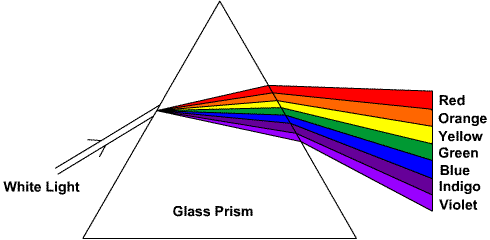
\includegraphics[width=0.5\textwidth]{img/dispersion.png}
	\caption{Dispersion along the edge of a glass prism}
	\label{fig:dispersion}
\end{figure}

One goal of this experiment is to characterize the prism of such a spectrometer. Opposite to the functionality mentioned above, the spectrometer can also be used to find the refractive index of the incoming at a certain wavelength by measuring the angle of deflection of the beam after travelling through the prism. In order to do that, the minimum angle of deflection $\delta_m$ must be found for a given wavelength. This is the angle at which the spectrum reverses its direction, meaning that the spectrum is steady when the minimum angle of deflection is reached. At this angle, the following relation holds:

\begin{equation}\label{eq:index}
n = \frac{\sin\alpha_1}{\sin\beta_1} = \frac{sin{\frac{\delta_m+\phi}{2}}}{\sin{\frac{\phi}{2}}}
\end{equation}

where $\alpha_1$ is the angle of incidence, $\beta_1$ the angle of reflection and $\phi$ the prism's wedge angle. This relation will be used to calculate the refractive indices of the prism at different wavelengths.\\

Additionally, if the prism's base length $a$ is known, the optical resolution $A$ of the prism can by found by using the derivative of the refractive index with respect to the wavelength $\frac{\dif n}{\dif \lambda}$:

\begin{equation}
A = a\cdot \frac{\dif n}{\dif \lambda}
\end{equation} 

\section{Experiment setup and execution}

\subsection{Used materials}
The materials used in this experiment are the following:
\begin{itemize}
\item a turntable, with an adjustable platform for the prism
\item a prism
\item a mercury vapor lamp
\item a collimator, mounted to the turntable, turnable 
\item a telescope, mounted to the turntable, turnable
\item an adjustable slit, mountable to the telescope
\end{itemize}

\subsection{Assembly and Execution}

\begin{figure}[H]
	\centering
  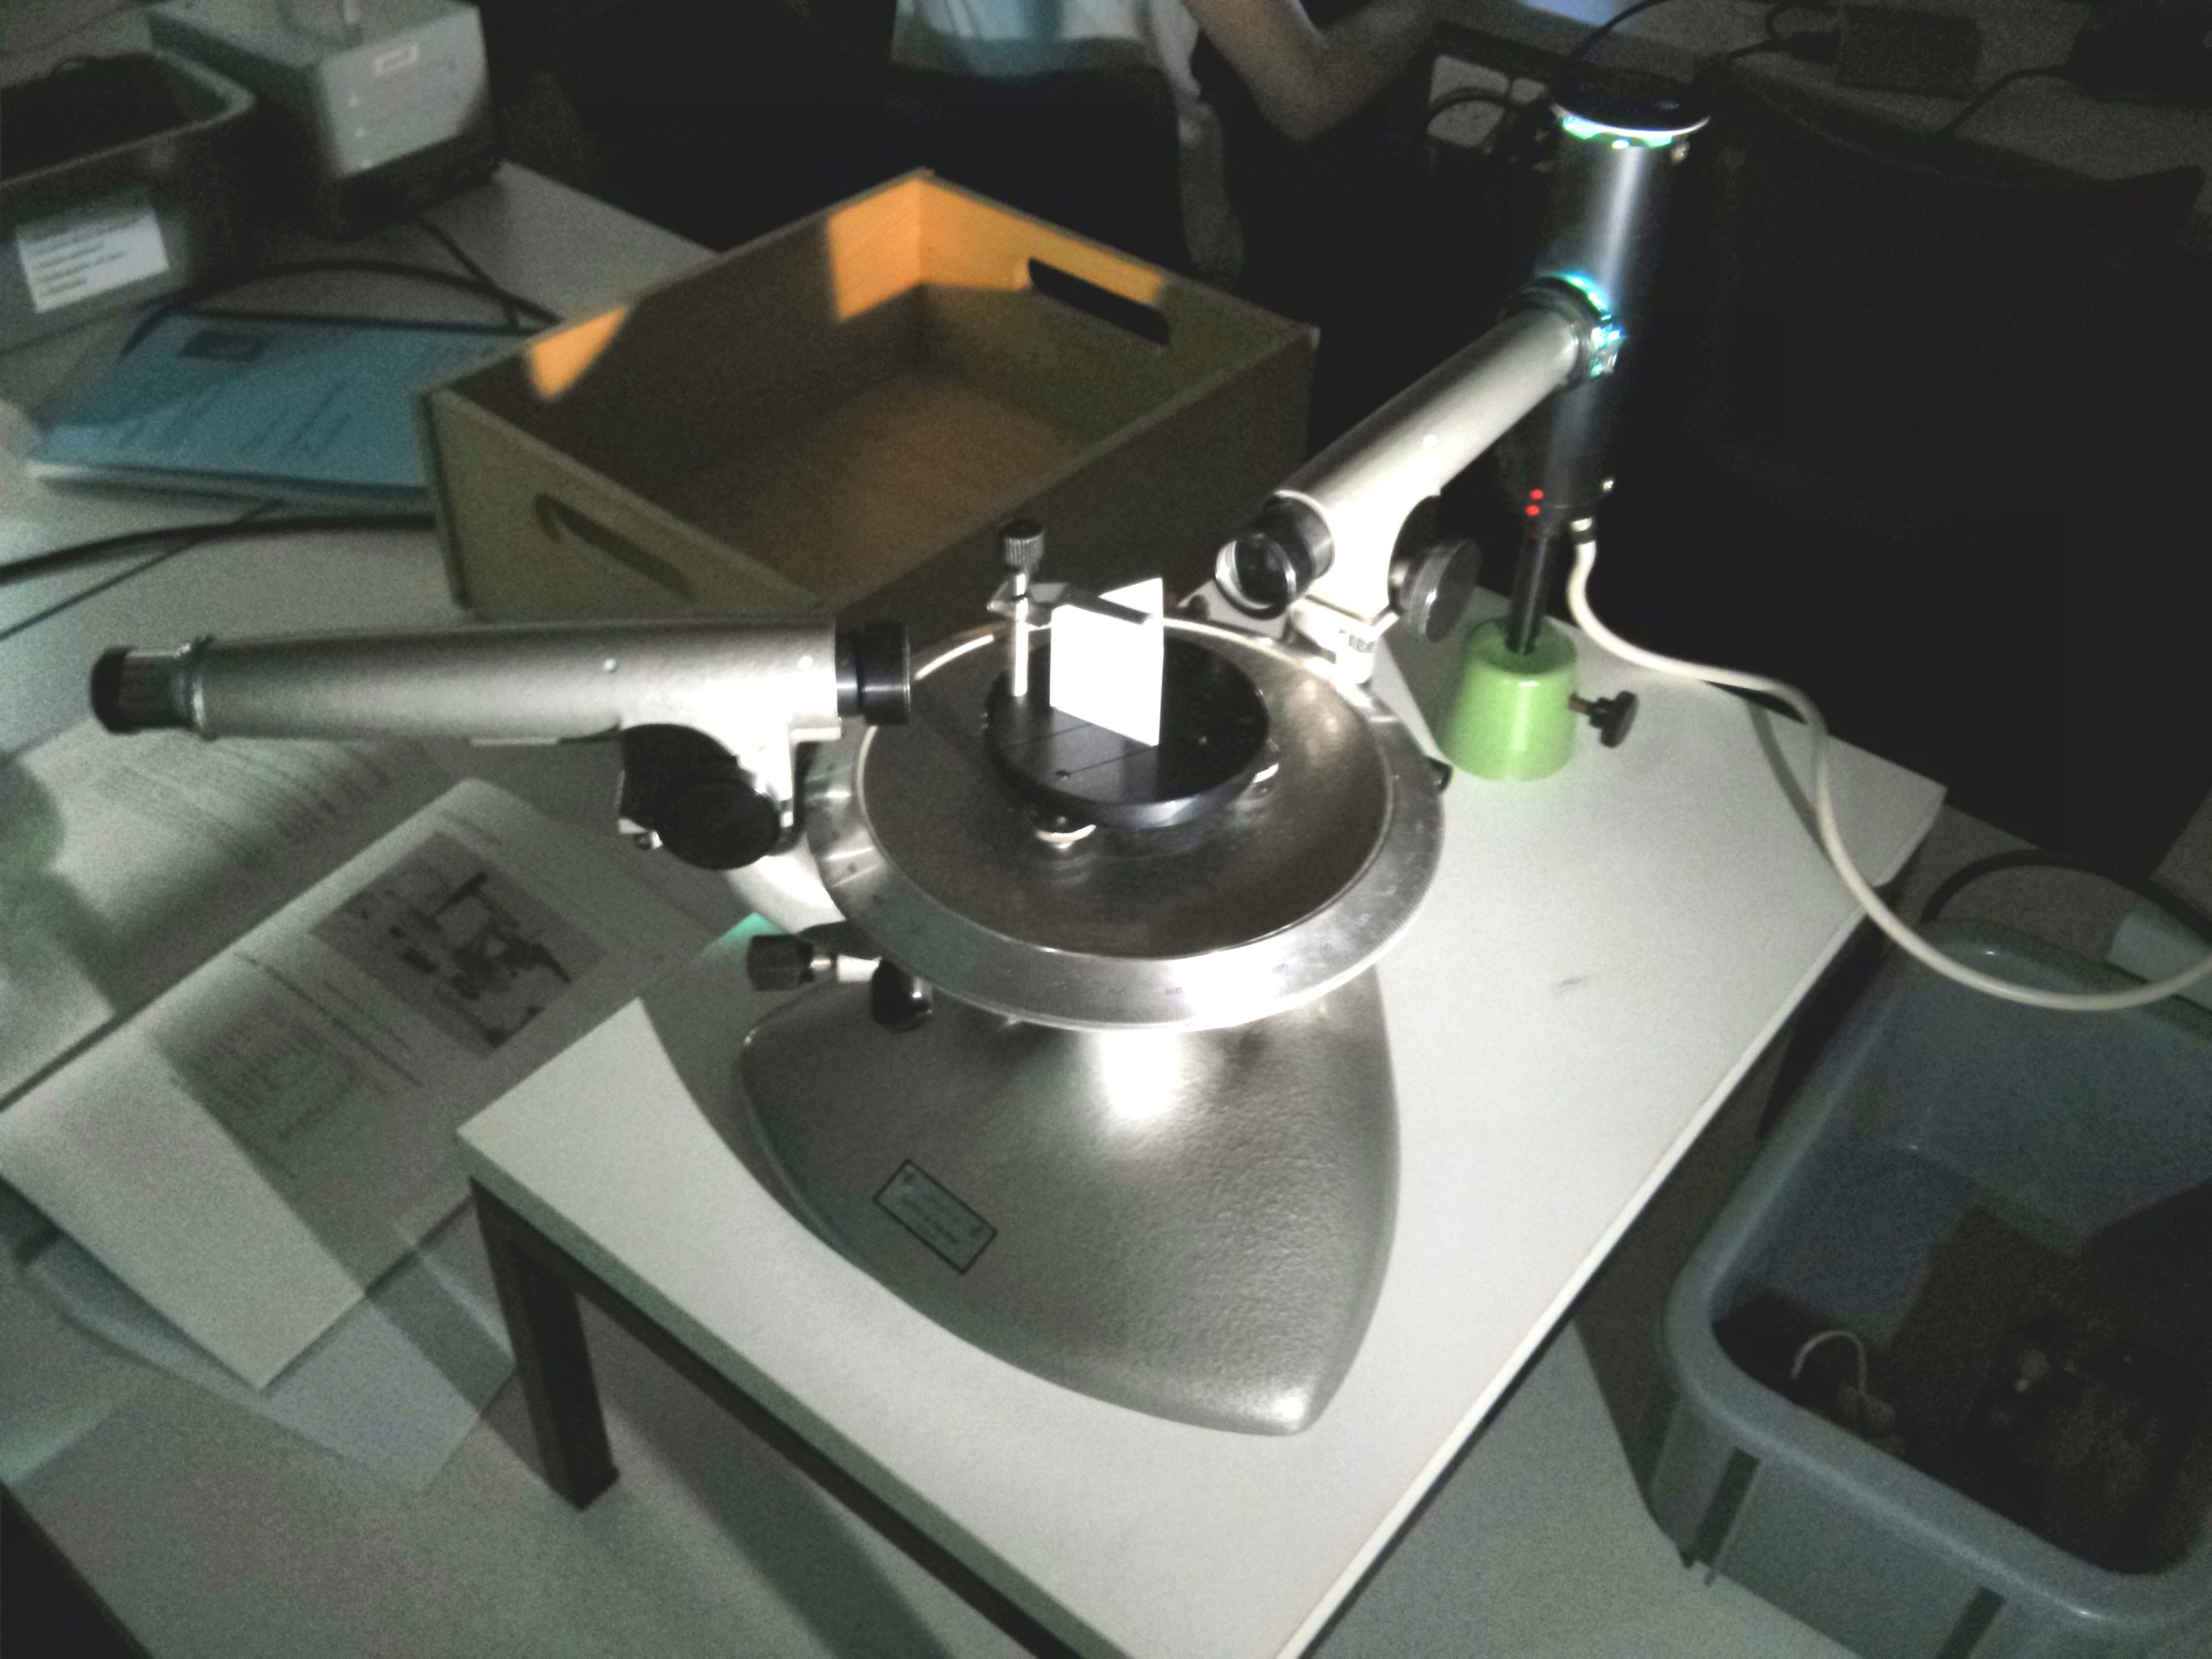
\includegraphics[width=0.9\textwidth]{img/assembly.jpg}
	\caption{Experiment Assembly}
	\label{fig:assembly}
\end{figure}

In the first measurement, we first adjusted the platform so the sides of the prism were exactly upright. Then, rotating the table to a position where one side faced the telescope, measuring the angle of the telescope and repeating the procedure for a second side, we measured the angle of the prism.
\\\\
For the second measurement, we lit up the vapor lamp and, rotating the platform, looked for the point where the spectral lines were minimally deflected. We measured that angle for each of the seven spectral lines stated in \cite[p. 159]{physcript13}. 
\\\\
For the third measurements, we mounted the adjustable slit on the telescope and closed it to the narrowest possible position where the yellow lines were still distinguishable, thus measuring the minimal base length. 
\section{Measurements}

\subsection{Minimal deflection}
\begin{figure}[H]
	\centering
  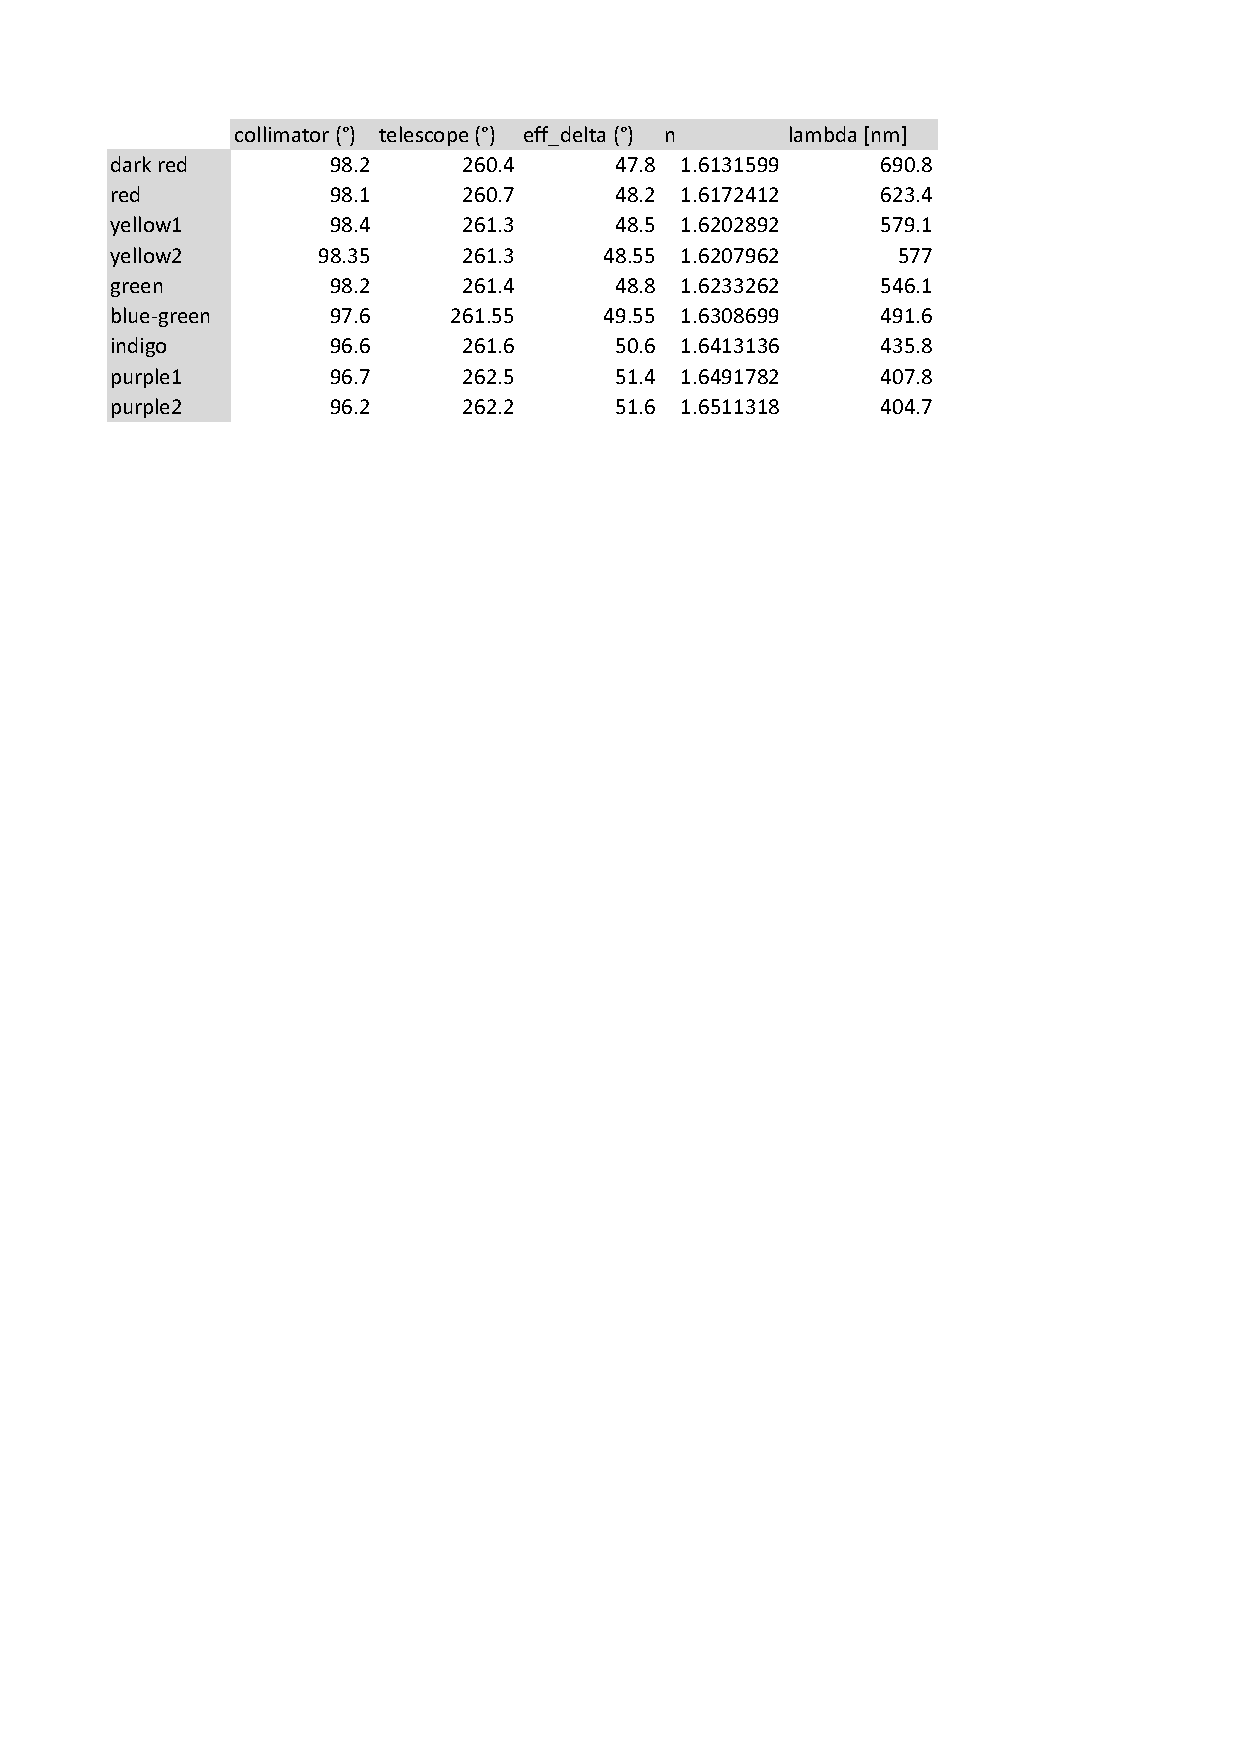
\includegraphics[width=0.9\textwidth]{diag/right.pdf}
	\caption{Minimum deflection angles on the right side}
	\label{fig:right}
\end{figure}

\begin{figure}[H]
	\centering
  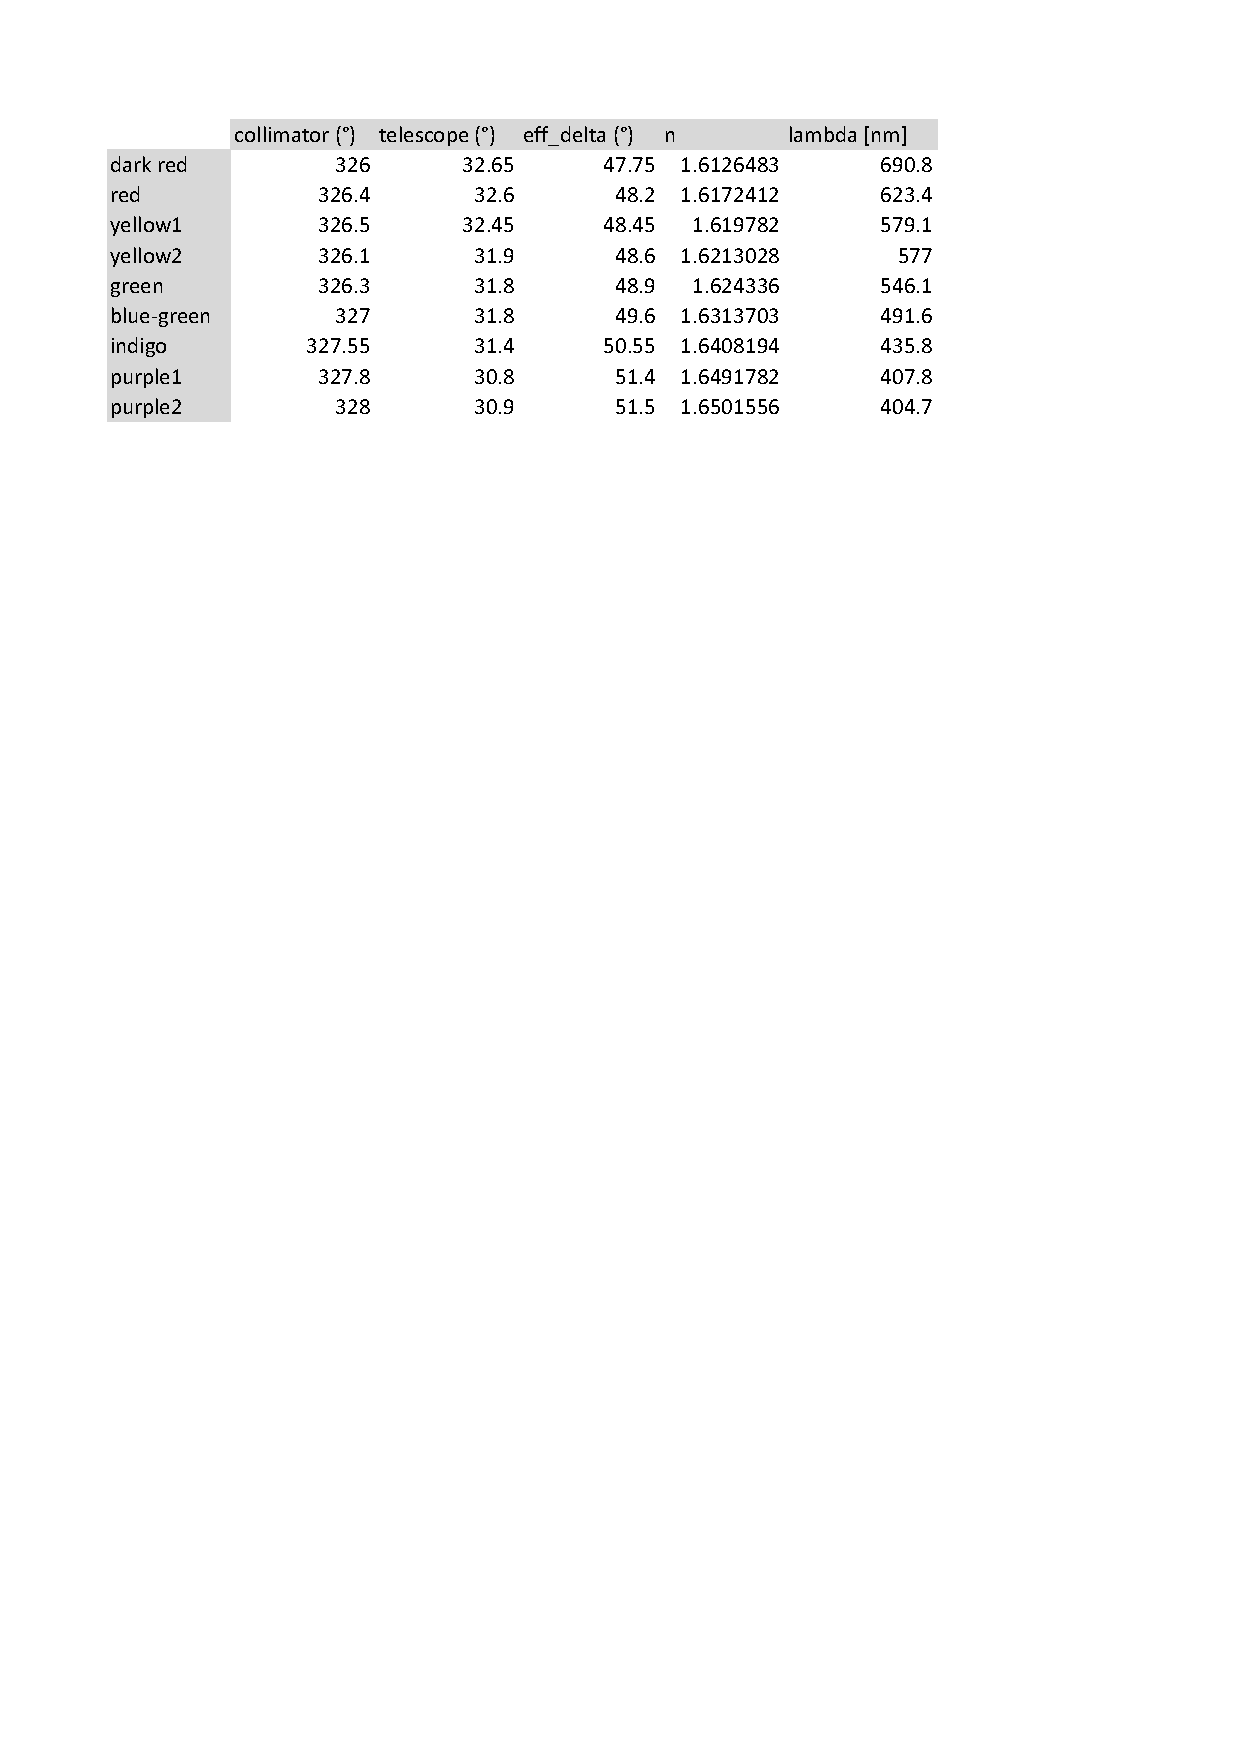
\includegraphics[width=0.9\textwidth]{diag/left.pdf}
	\caption{Minimum deflection angles on the left side}
	\label{fig:left}
\end{figure}
\subsection{Minimal Base Length}
We measured a minimal slit width $x$ of:
\begin{equation}
	x = 0.76\unit{mm}
\notag
\end{equation}

\section{Analysis and Discussion}

\subsection{Wedge Angle of the Prism}

Our measurements for the wedge angle of the prism yielded the following:
\begin{equation}
	\phi = \ang{60.2}
\notag
\end{equation}
We think the footprint of the used prism is an equilateral triangle, although we have no coherent proof for our assumption.

\subsection{Minimal Deflection}
\begin{figure}[H]
	\centering
  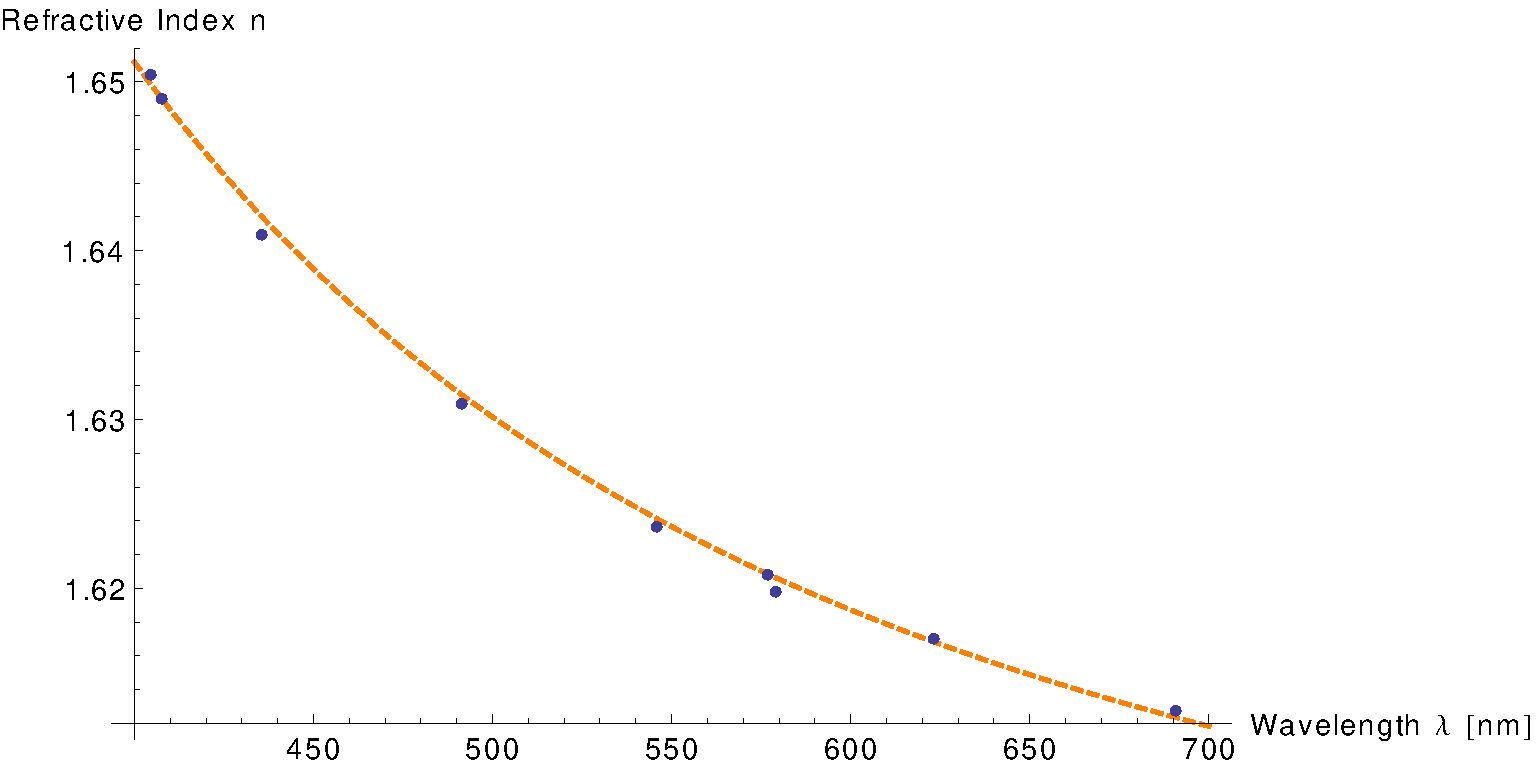
\includegraphics[width=0.9\textwidth]{diag/meas_and_fit.pdf}
	\caption{Calculated refractive indices $n$ plotted against the wavelength $\lambda$ of the spectrum}
	\label{fig:meas_and_fit}
\end{figure}
As predicted by theory, the refractive Index $n$ is higher for lower wavelengths and lower for higher wavelengths. Furthermore, the obtained values fall in line with values for different kinds of glass, which we think is a strong indication that our values are reasonable.

\subsection{Minimal Base Length}

Using formula \ref{slit} ... we can do something, can't we?


\section{Conclusion}

\begin{thebibliography}{9}

\bibitem{physcript13}
  Peter Wurz,
  \emph{Anleitung zum Physikpraktikum}
  FS2013

\end{thebibliography}

\end{document}
